\subsection{Gluing Column Extrusions together with Strip Connectors}
\label{sec:strip_connectors}
Now that all the column extrusions $\left\{ \mathcal C^{(i)} \right\}$ have the same evolution time,
we would like to glue them together into a continuous strip of paper.
In order to achieve this, we consider the time-axis boundaries of $\mathcal C^{(i)}$ (red line in Figure~\ref{fig:level_shift},~\ref{fig:up_down}).
First, note that the boundaries always lie on the same plane, corresponding to the zero level.
We will constrain this to be on the plane $z=0$. Now, let us consider the motion of the boundary on this plane.

\graphicspath{{./figures/}}
\begin{wrapfigure}[16]{r}{0.27\textwidth}
    \vspace{-2.8em}
    \def\svgwidth{0.27\textwidth}
    \input{./figures/boundaries.pdf_tex}%
    \caption{Boundaries of adjacent column extrusions ($D_j = 8\varepsilon$). $\phi$ denotes a zero distance.}
    \label{fig:boundaries}
    %\vspace{-1.8em}
\end{wrapfigure}
\begin{itemize}
    \item During the horizontal evolution of any row $j$, both boundaries move along the positive $y$-axis with unit velocity
          (Figure~\ref{fig:level_shift0},~\ref{fig:level_shift3},~\ref{fig:level_shift4},~\ref{fig:up_down0},~\ref{fig:up_down3},~\ref{fig:up_down4}).
%\end{itemize}
%\begin{itemize}[resume, before = \vspace*{-\dimexpr\topsep+\partopsep\relax}]
    \item During the vertical transition from row $j$ to $j+1$, both boundaries move back and forth along the $x$-axis with unit velocity.
          (Figure~\ref{fig:level_shift1},~\ref{fig:level_shift2},~\ref{fig:up_down1},~\ref{fig:up_down2}).
          We can divide the vertical transition into $k = D_j/(2\varepsilon)$ intervals of length $2\varepsilon$.
          Each of these interval segments is either a up-shift, a down-shift, or a up-down gadget.
    \begin{itemize}
        \item In the first half of each interval ($\varepsilon$ time), the left and right boundaries move towards each other;
              i.e., the left boundary moves along the positive $x$-axis,
              and the right boundary moves along the negative $x$-axis for a distance of $\varepsilon$.
        \item In the second half of each interval, the left and right reverse velocities, and return to their original positions.
        \item After $D_j$ time, the boundaries return to their original positions, and resume their movement in the positive $y$ direction.
    \end{itemize}
\end{itemize}

We will attempt to construct a cross section sequence whose left and right boundaries
line up with the adjacent column extrusion boundaries shown in Figure~\ref{fig:boundaries}.
Notice that the distance between \emph{corresponding points} on the boundaries varies between $0$ and $2\varepsilon$.
So, the connector strip must have width at least $2\varepsilon$.

We outline a construction of a $2\varepsilon$ width strip, as shown in Figure~\ref{fig:connector_cross_section}.
During horizontal evolution, the cross section comprises of two vertical segments, each of length $\varepsilon$,
which move along the same trajectory in the positive $y$-direction
(during horizontal evolution Figure~\ref{fig:column_connector0},~\ref{fig:column_connector10}).
Now, consider a transition of length $D_j$ divided into intervals of length $2\varepsilon$,
each of which evolves according to Figure~\ref{fig:connector_cross_section}.
\begin{itemize}
    \item The vertical segments move outwards with unit velocity to match the outward moving boundaries of the adjacent strips.
          An upwards moving horizontal segment of length zero is created between the two existing segments (Figure~\ref{fig:column_connector1}).
\end{itemize}

\begin{itemize}[resume, before = \vspace*{-\dimexpr\topsep+\partopsep\relax}]
    \item After time $\varepsilon$, the length of the vertical segments become zero,
          and the horizontal segment spans the $2\varepsilon$ gap between the column boundaries (Figure~\ref{fig:column_connector2}).
          Notice that that the boundary of the connector maintains its $z$ coordinate (Figure~\ref{fig:connector_cross_section}).
    \item Then the connector segments reverse velocities, and retrace their path for $\varepsilon$ time (Figure~\ref{fig:column_connector3}),
          until the vertical segments become length $\varepsilon$, and the horizontal segment disappears (Figure~\ref{fig:column_connector4}).
    \item The entire process repeats $D_j/(2\varepsilon)$ times (Figure~\ref{fig:column_connector5},~\ref{fig:column_connector6},~\ref{fig:column_connector7}).
\end{itemize}

The completed connector gadget is shown in Figure~\ref{fig:column_connector8},~\ref{fig:column_connector9}.
We show the \emph{connector gadget} attached to an \emph{up-shift gadget} in Figure~\ref{fig:column_connector7},~\ref{fig:column_connector10}.
\graphicspath{{./figures/}}
\begin{figure}[!h]
    \def\svgwidth{1.0\textwidth}
    \input{./figures/connector_cross_section.pdf_tex}%
    \caption{
    Cross section evolution of column connector gadget.
    }
    \vspace{-1.5em}
    \label{fig:connector_cross_section}
\end{figure}

\begin{figure}[!htb]
\graphicspath{{figures/column_connector}}
    \centering
    \subfloat[Initial height.]{
        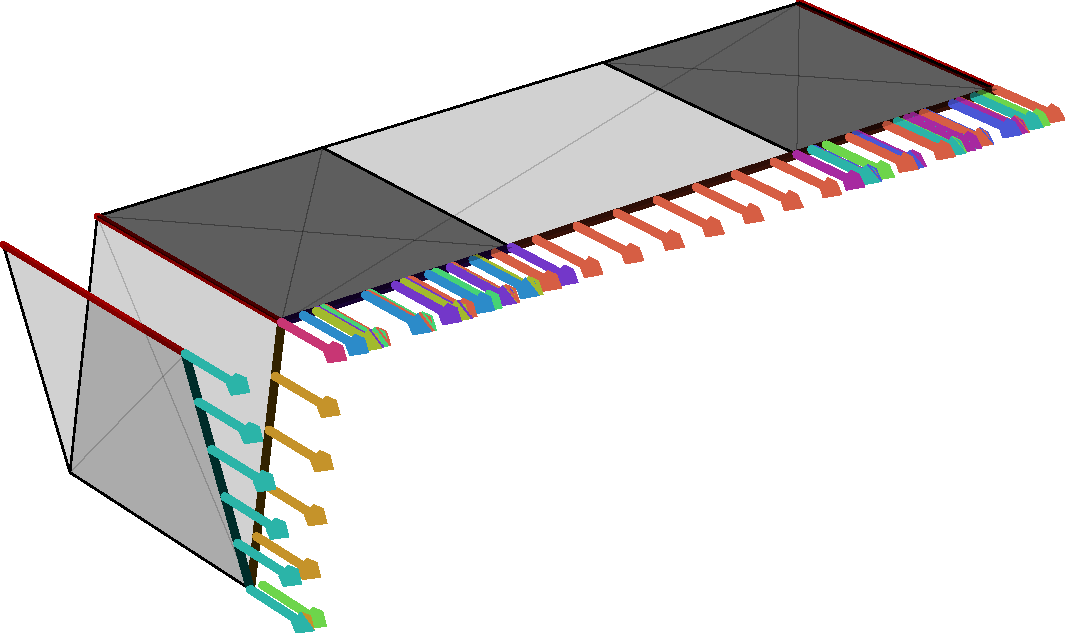
\includegraphics[width=0.23\textwidth]{figures/column_connector/column0.pdf}
    }%
    \subfloat[Connector moves outwards.]{
        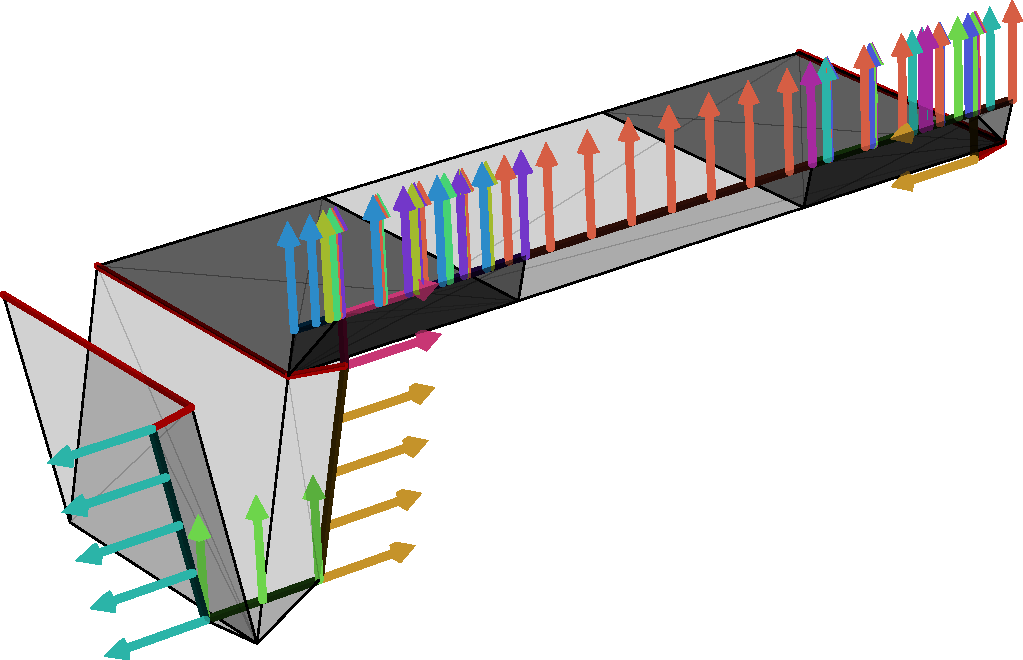
\includegraphics[width=0.21\textwidth]{figures/column_connector/column1.pdf}
    %}
    %\subfloat[]{
        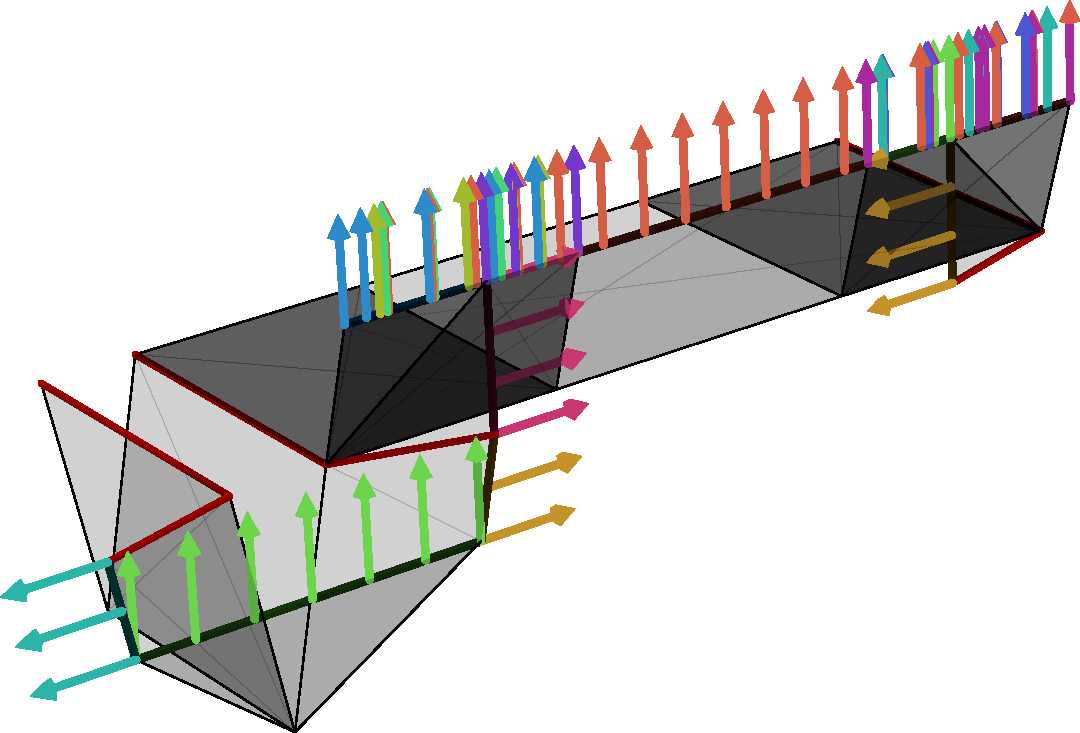
\includegraphics[width=0.21\textwidth]{figures/column_connector/column2.pdf}
    }%
    \subfloat[Connector at maximum width.]{
        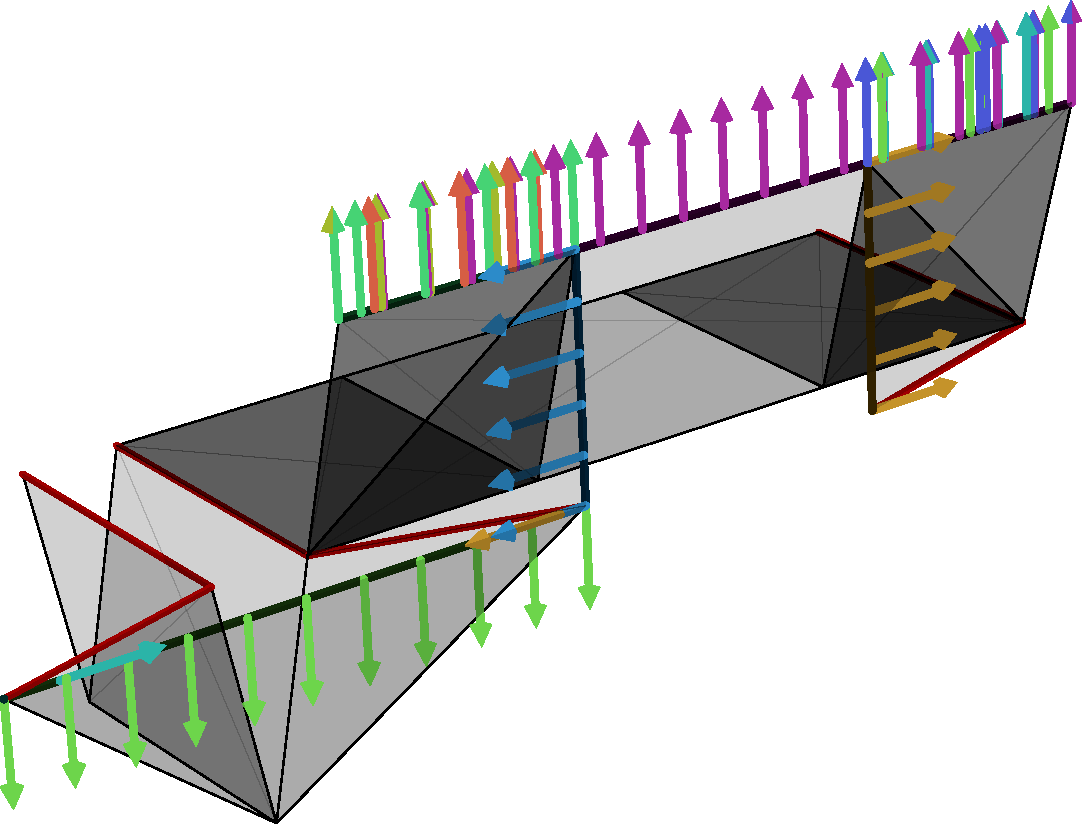
\includegraphics[width=0.24\textwidth]{figures/column_connector/column3.pdf}
    }%

    \subfloat[Connector moves inwards.]{
        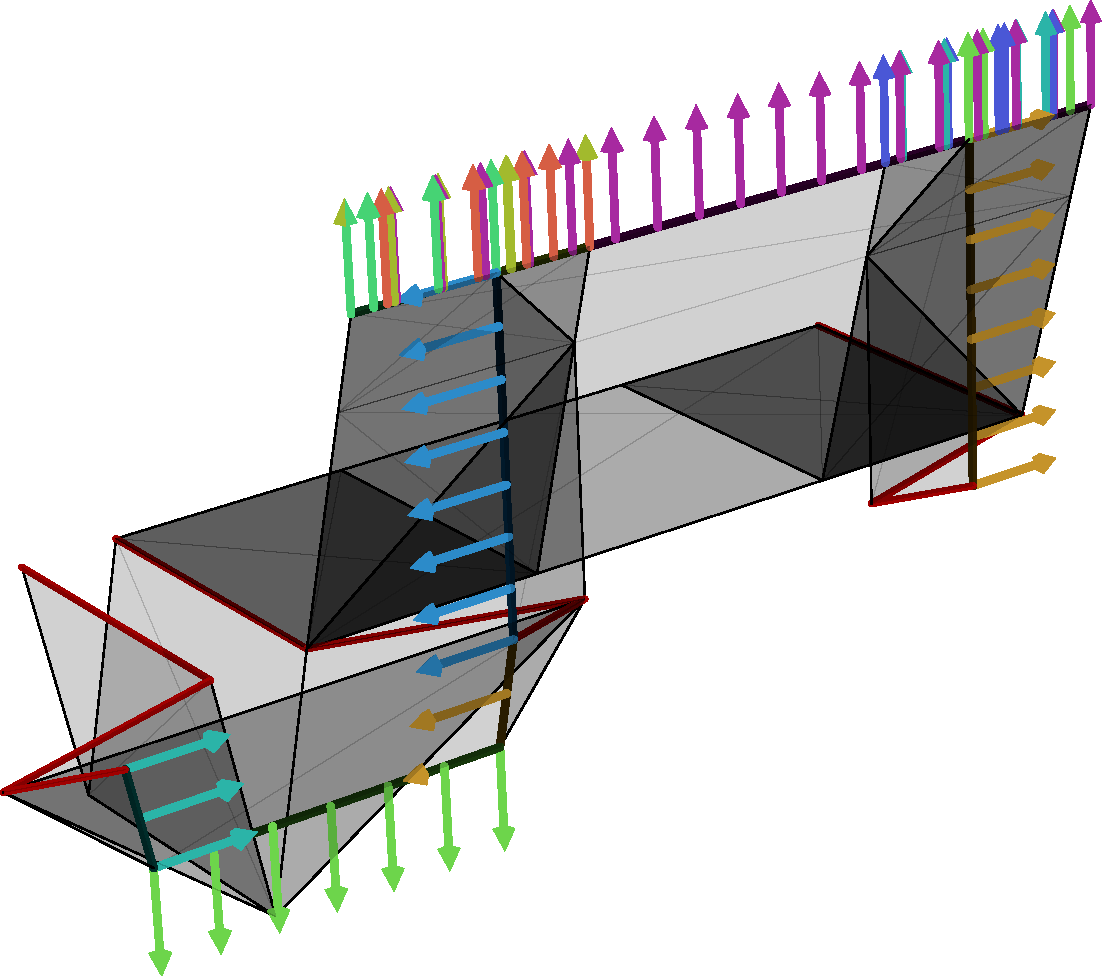
\includegraphics[width=0.23\textwidth]{figures/column_connector/column4.pdf}
    %}
    %\subfloat[]{
        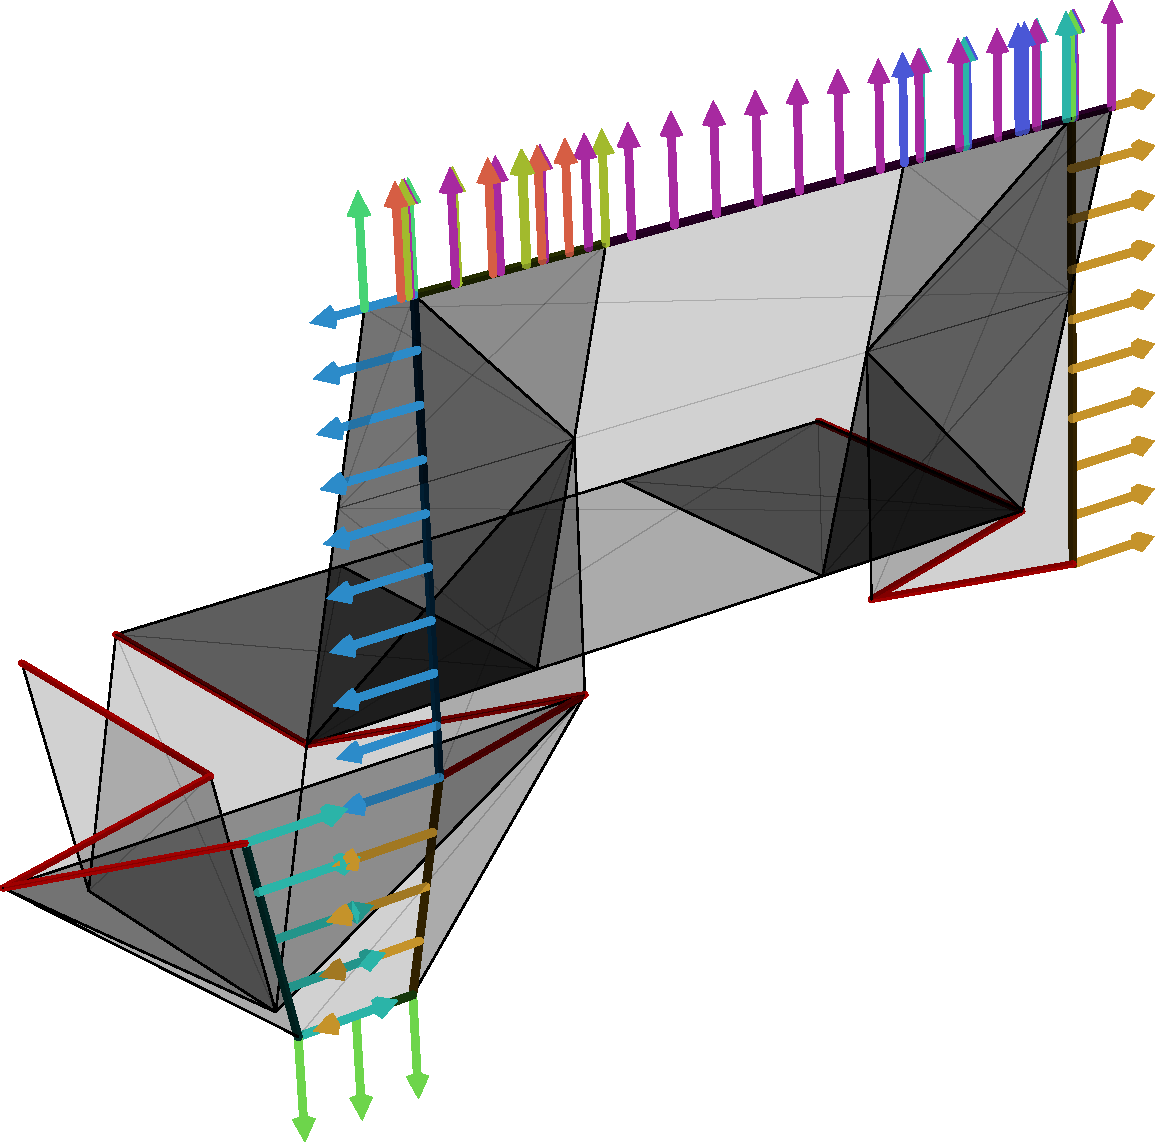
\includegraphics[width=0.23\textwidth]{figures/column_connector/column5.pdf}
    }%
    \subfloat[Back to \textbf{(a)}.]{
        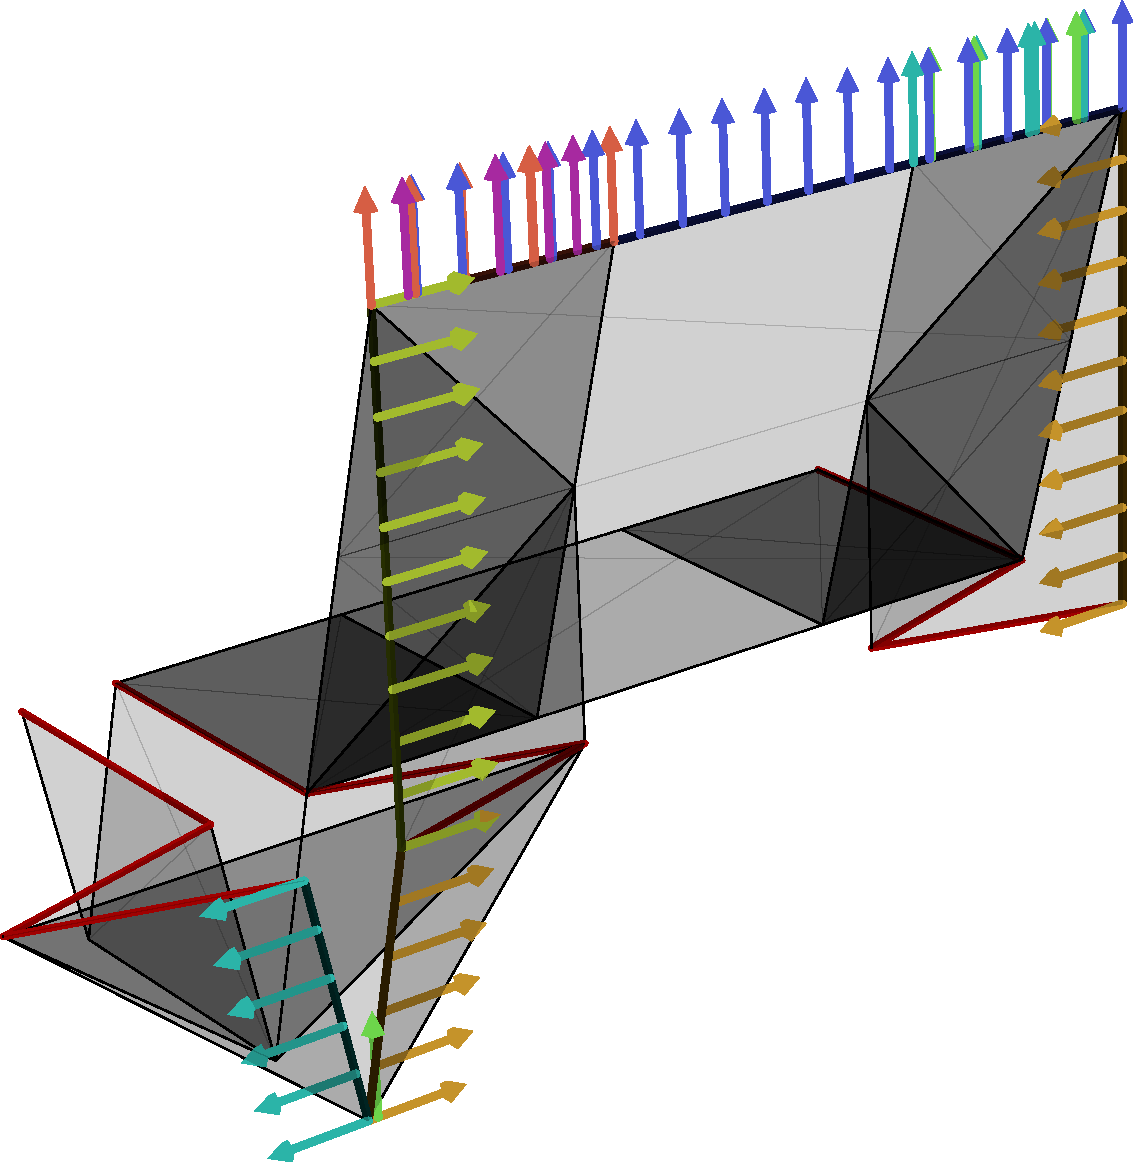
\includegraphics[width=0.23\textwidth]{figures/column_connector/column6.pdf}
    }%
    \subfloat[Same as \textbf{(b)}.]{
        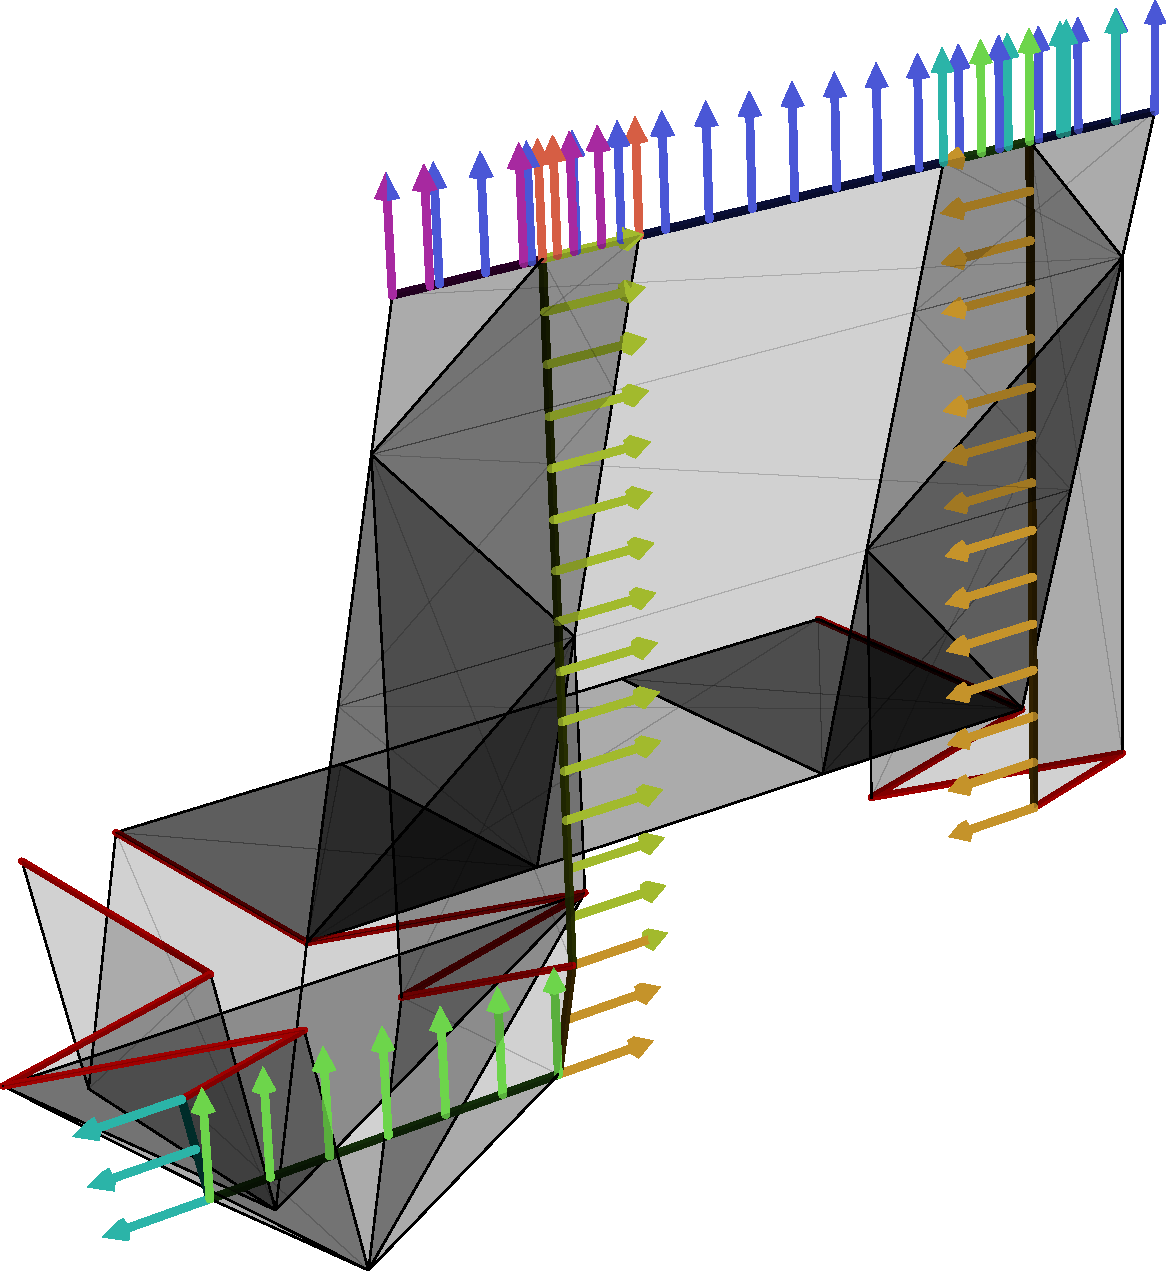
\includegraphics[width=0.23\textwidth]{figures/column_connector/column7.pdf}
    }%

    \subfloat[Same as \textbf{(d)}.]{
        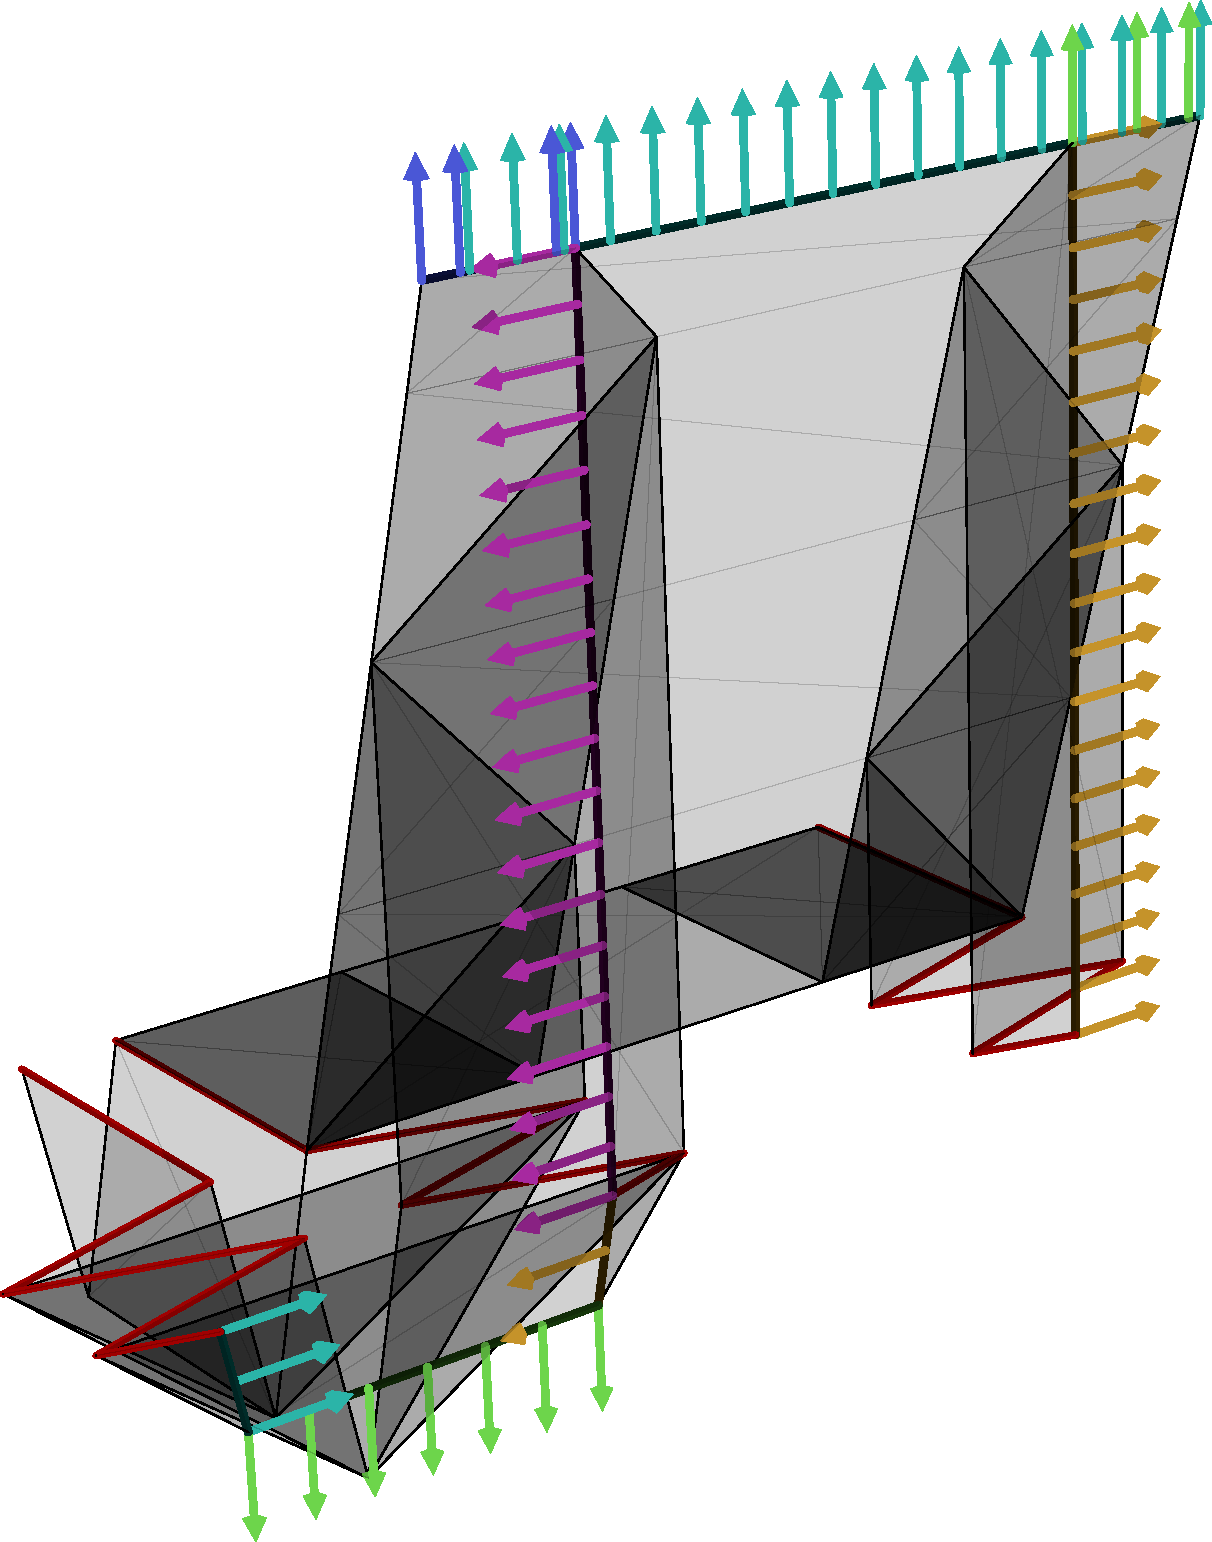
\includegraphics[width=0.29\textwidth]{figures/column_connector/column8.pdf}
    }%
    \subfloat[Level shift complete, and next level continues.]{
        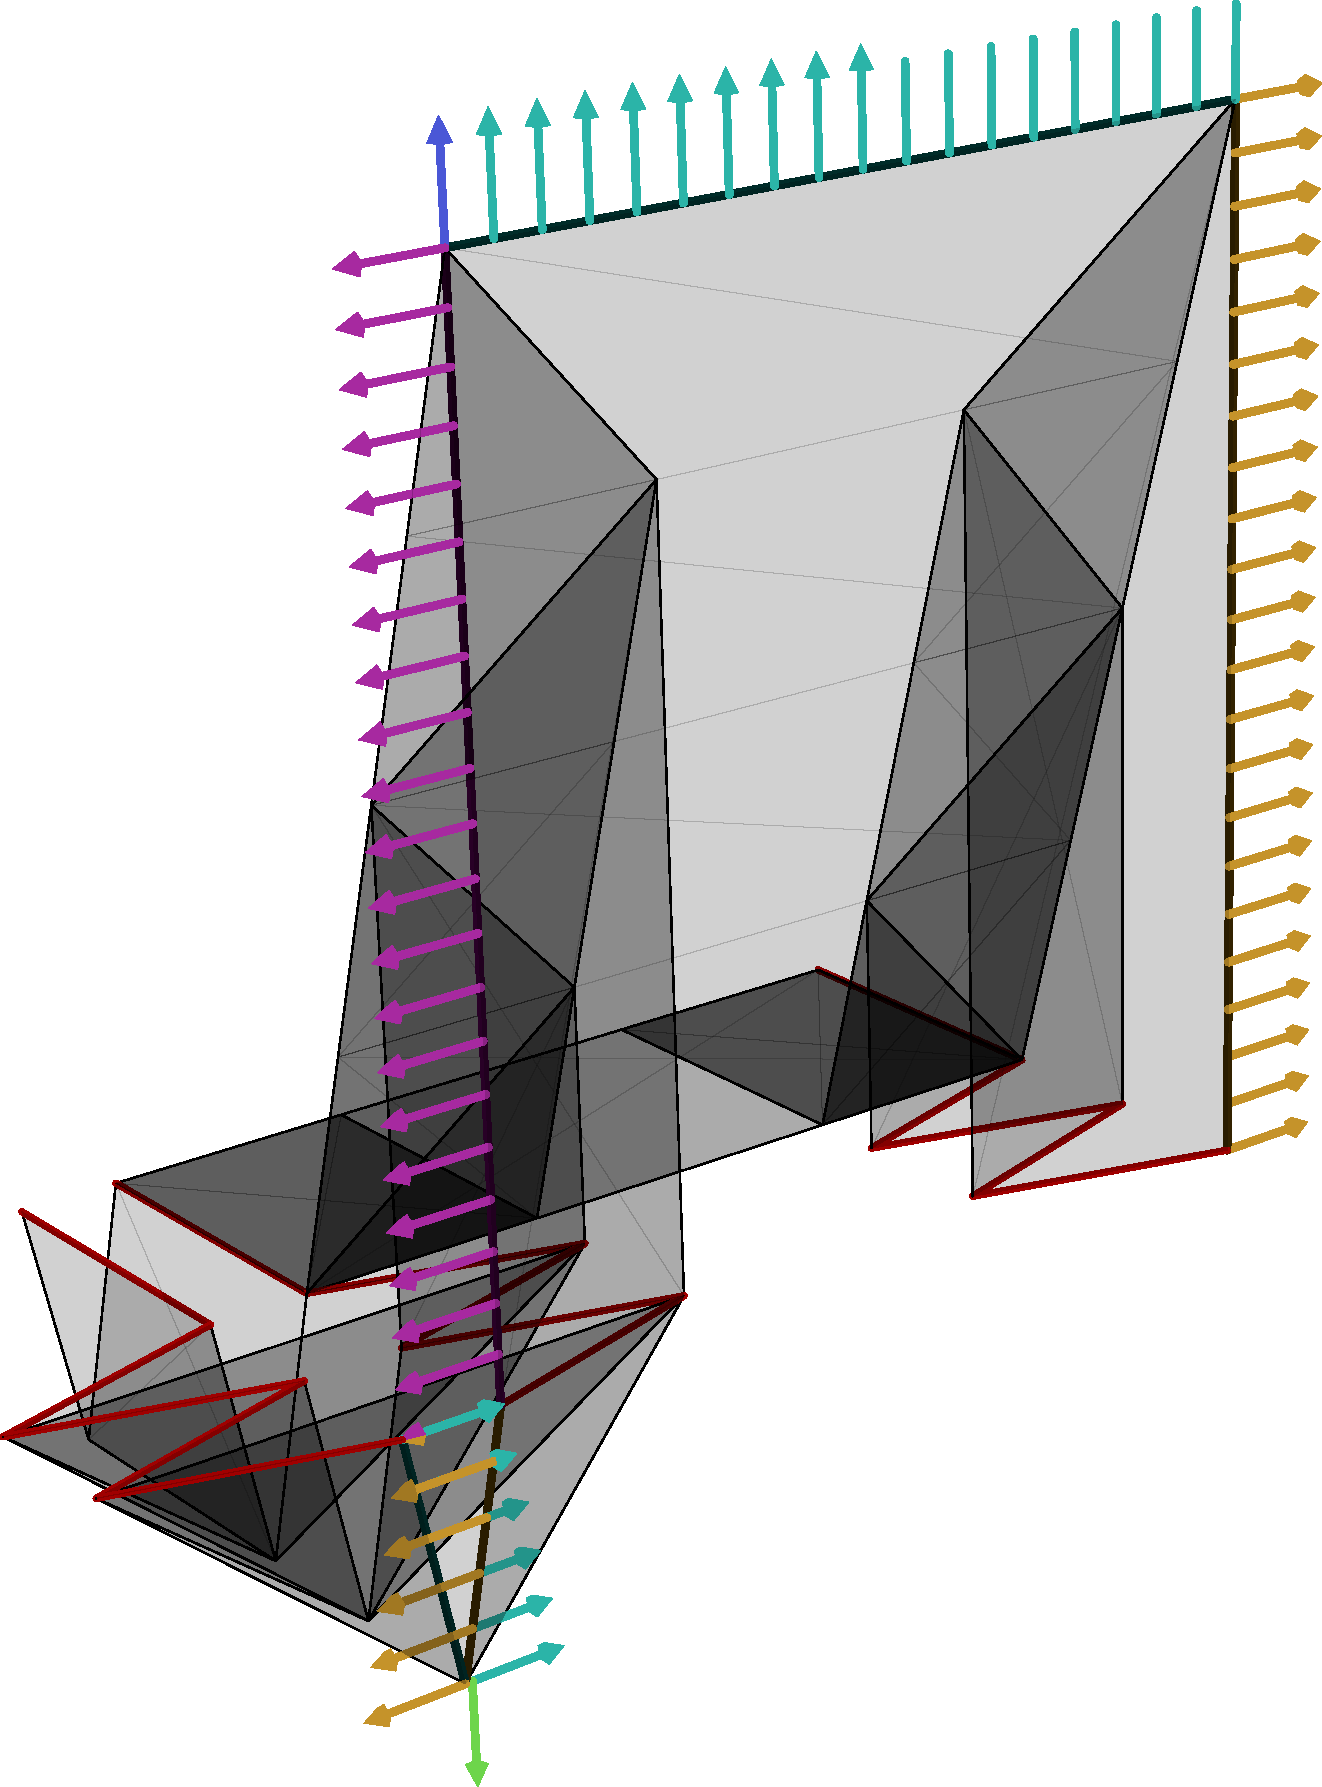
\includegraphics[width=0.29\textwidth]{figures/column_connector/column9.pdf}
    %}
    %\subfloat[Column and connector]{
        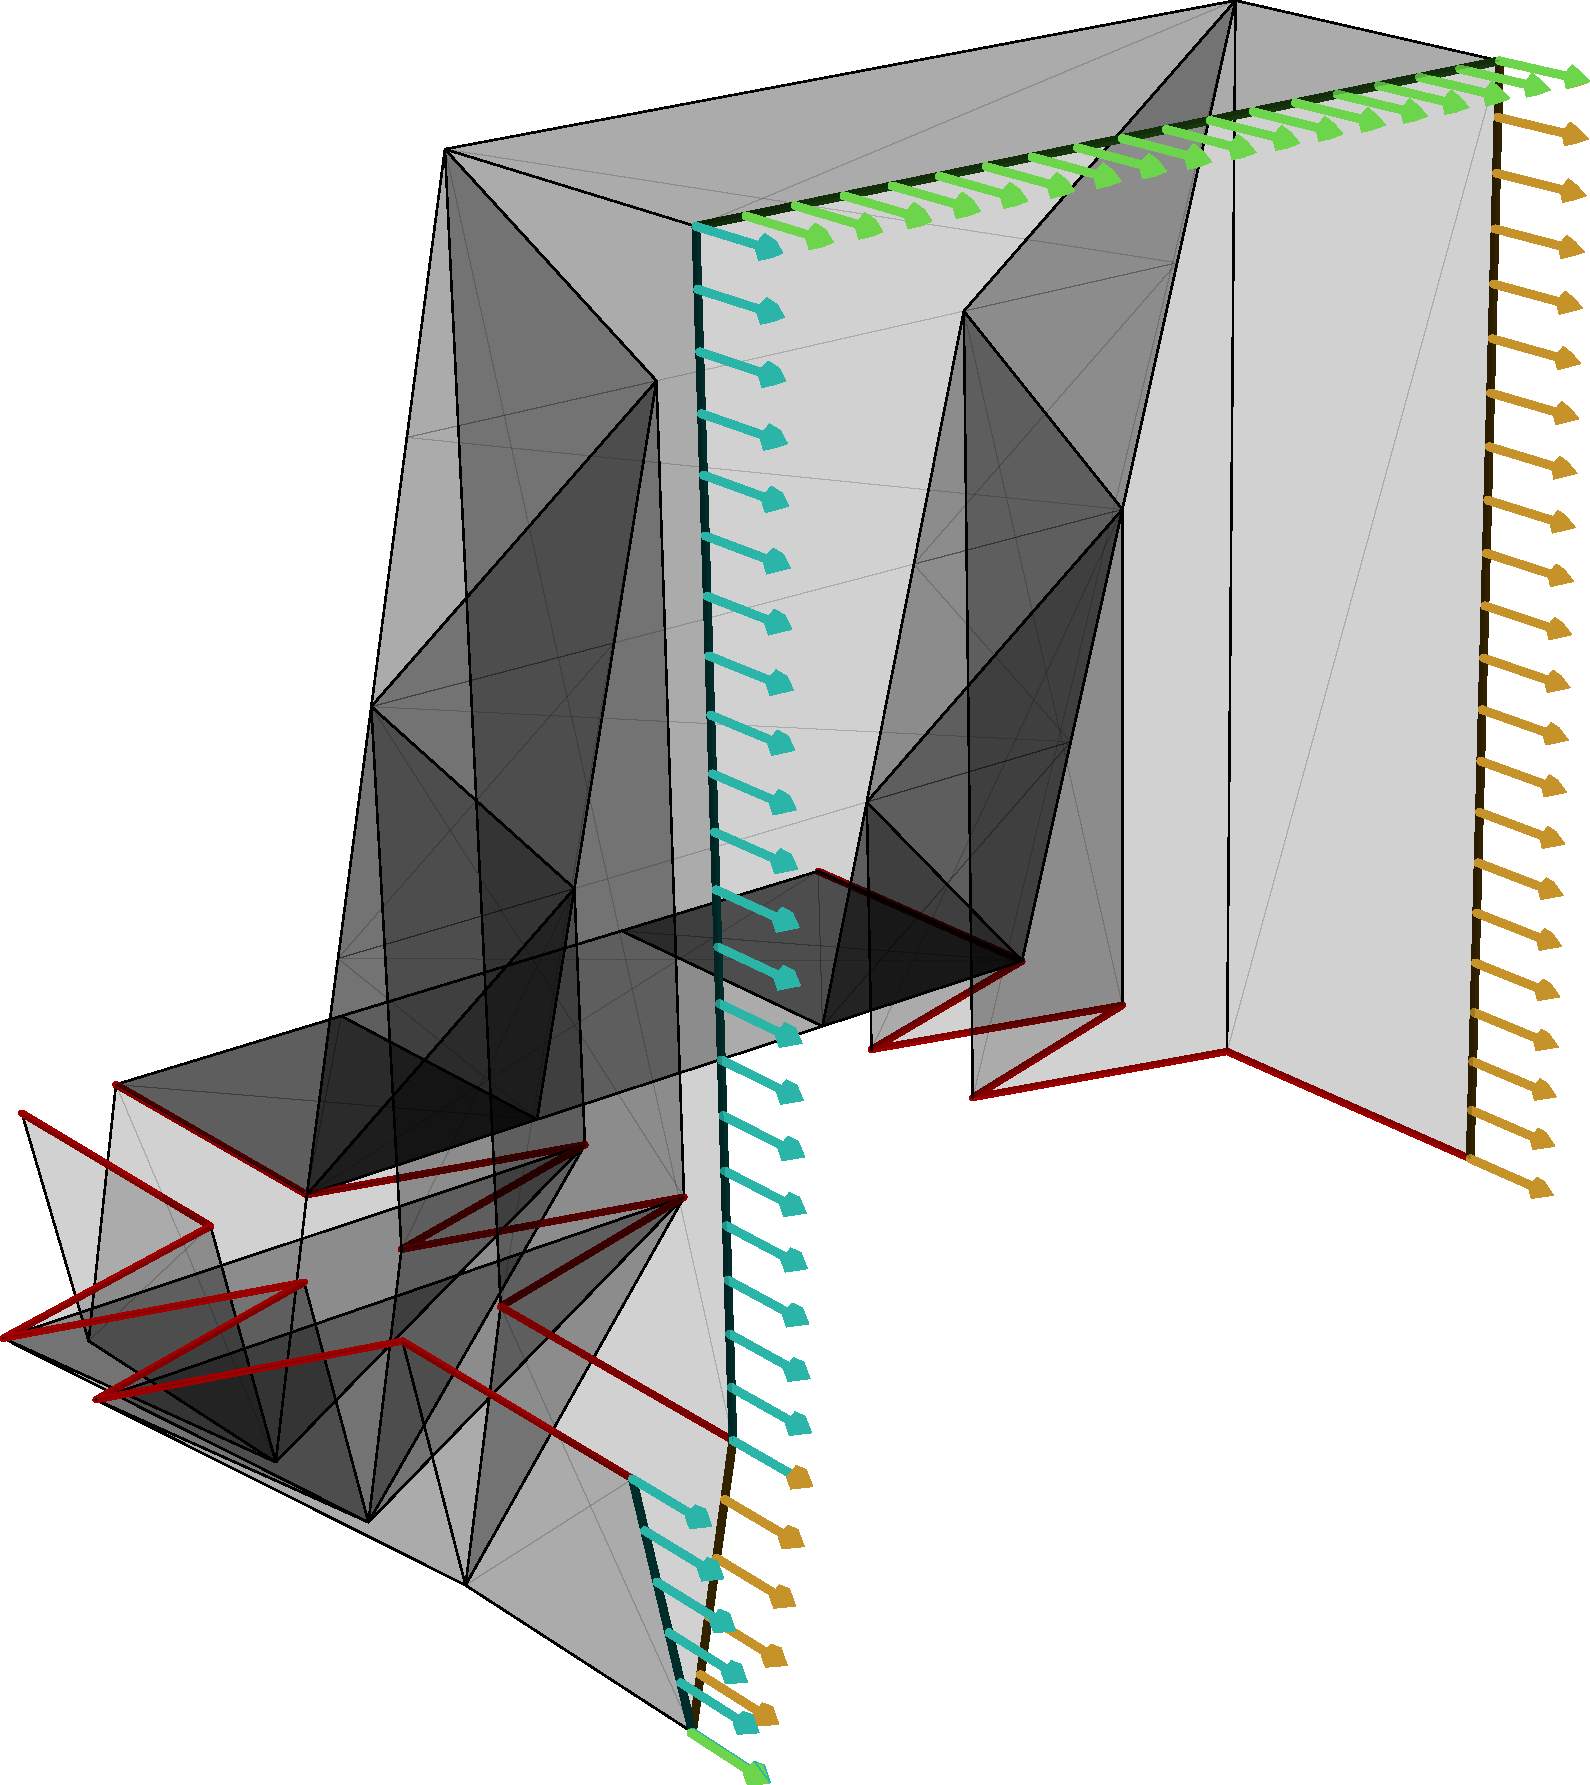
\includegraphics[width=0.34\textwidth]{figures/column_connector/column11.pdf}
    }%

    \subfloat[Connector gadget.]{
        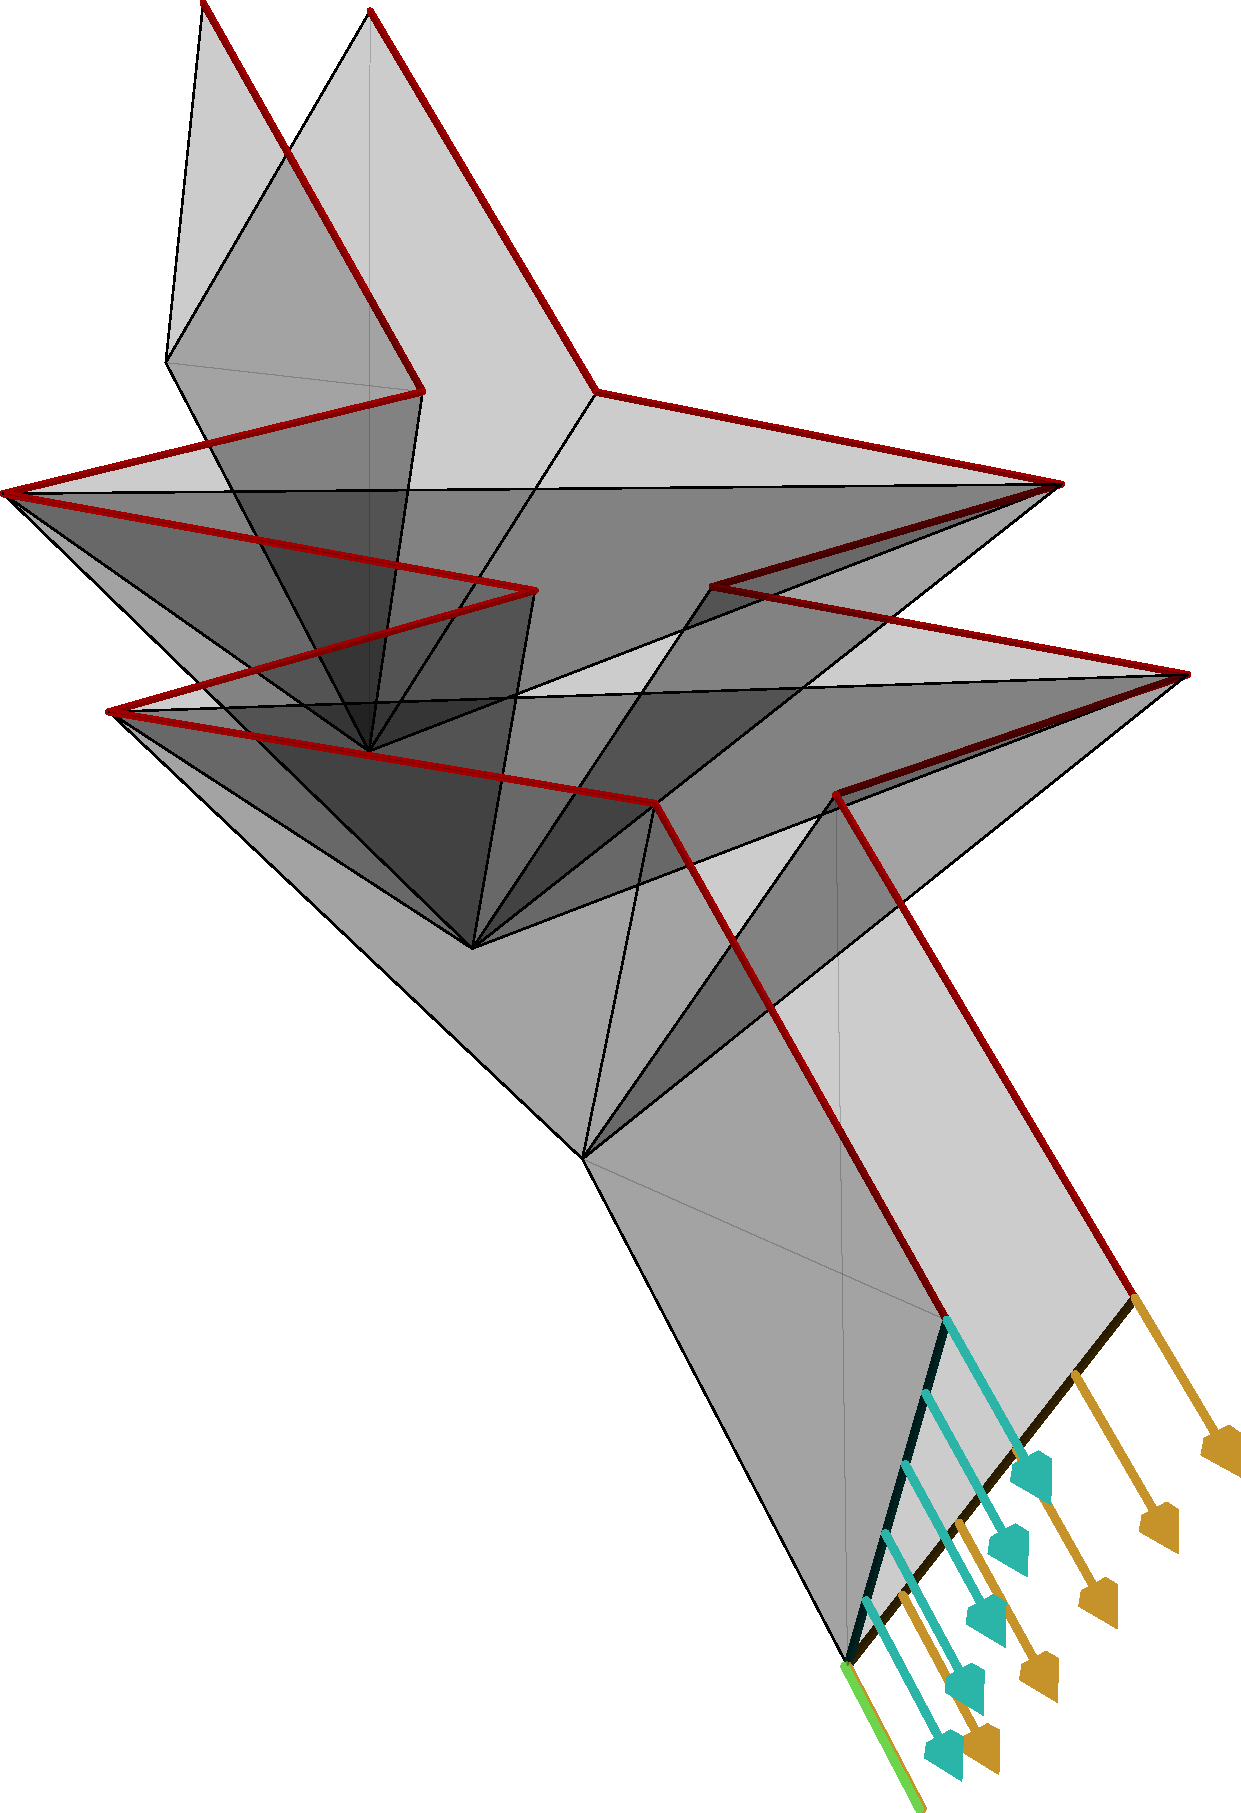
\includegraphics[width=0.31\textwidth]{figures/column_connector/connector0.pdf}
    }%
    \subfloat[Side view.]{
        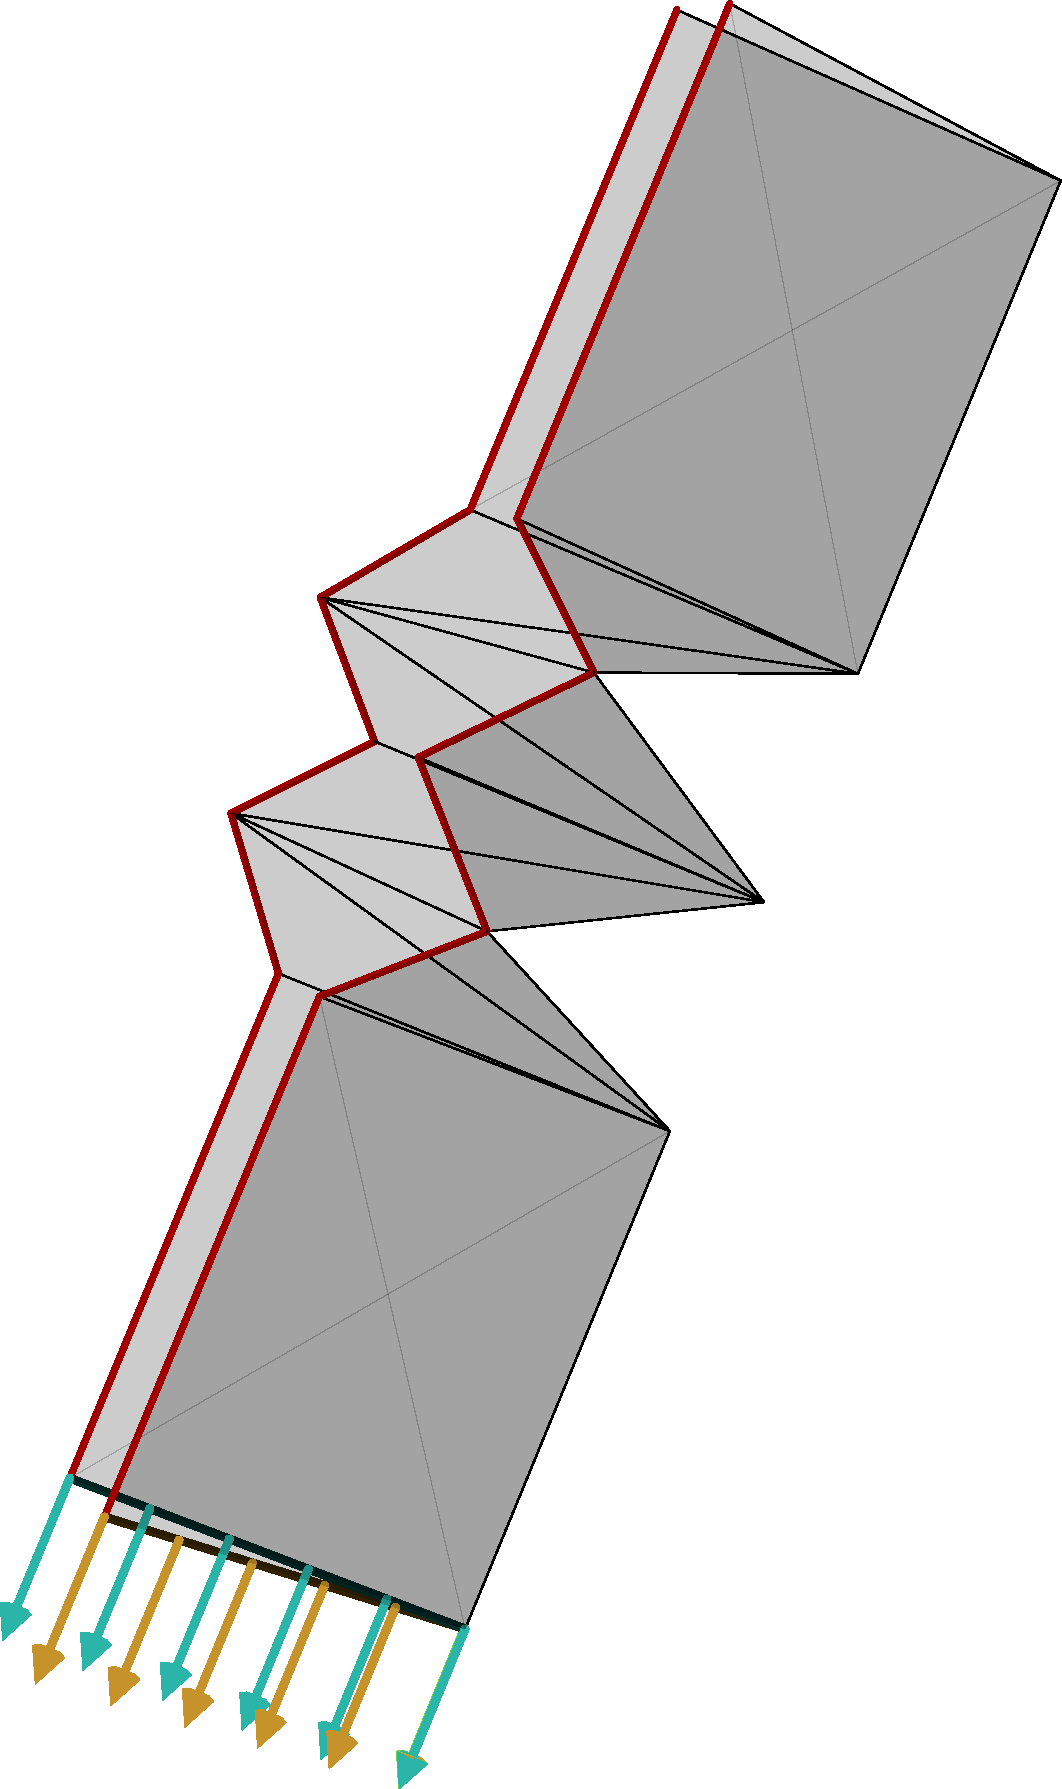
\includegraphics[width=0.27\textwidth]{figures/column_connector/connector1.pdf}
    }%
    \subfloat[Flat folded state.]{
        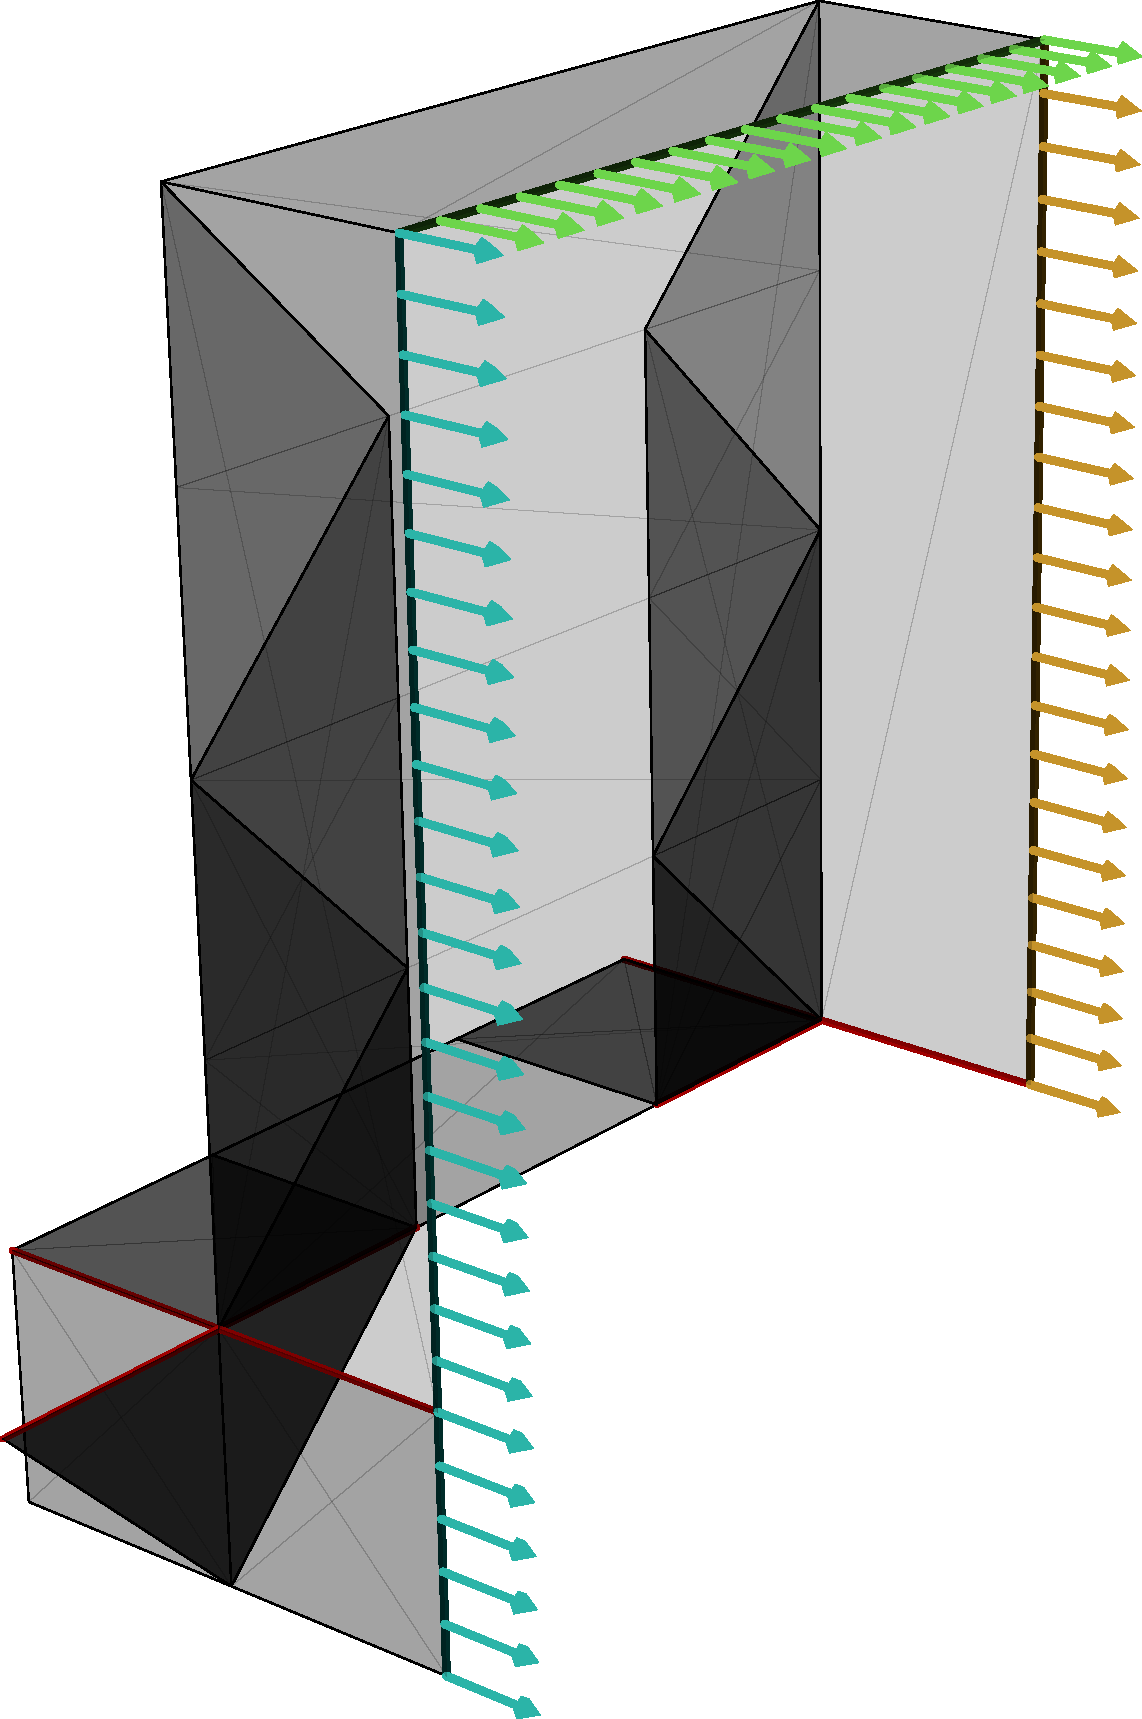
\includegraphics[width=0.31\textwidth]{figures/column_connector/column_connector0.pdf}
    }%
    \caption{
    Column gadget attached to a single column connector gadget.
    The red line demarcates the interface between the two gadgets.
    }
    \label{fig:column_connector}
    \vspace{-20pt}
\end{figure}
\clearpage


%\subsubsection{Alignment with Level Shifts}
%\label{sec:alignment_with_level_shifts}

